\subsection{$180\degree$ Turn}
\label{subsec:180}

When optimizing a $180\degree$ turn the radius plays a big role, as can be seen in Figures \ref{fig:turns_cur_180deg_pos} and \ref{fig:turns_cur_180deg_camera}. The figures show optimizations of six $180\degree$ turns with radius ranging from $300$m to $50$m.

Unsurprisingly, broader turns give better solutions. For the turn with $300$m radius the tracking is very good. And while the tracking is not as good for the turns with $250$m and $200$m, they return a smooth stable path that puts the camera centre not too far away from the path. Notice in Figures \ref{fig:turns_cur_180deg_camera_250} and \ref{fig:turns_cur_180deg_camera_200} that the tracking not only is worse throughout the turn, there is also more overshoot at the end of the turn. The MPC most likely accepts this overshoot as the deviance from the camera path is a lower cost than using more control input to sharpen the turn. Figure \ref{fig:turns_cur_180deg_roll} shows that the $250$m and $200$m turns already have higher roll angles, and opposed to the $300$m turn they do not flatten out during the turn.

For the radii $150$m, $100$m, and $50$m the result is not as good. For the turns with $150$m and $100$m radius the result is similar to previous paths where the path is too sharp: the MPC uses roll to compensate for the sharp turn, which causes the aircraft to enter a spiral. In Figure \ref{fig:turns_cur_180deg_pos_100} it may appear as the aircraft is about to recover and continue tracking the ground path, but the height plots show that at this point the aircraft is only about $20$m above ground and still descending.

For the $50$m turn in Figure \ref{fig:turns_cur_180deg_pos_50} the MPC fails differently. About $250$m before the turn even begins the aircraft drifts off to the left, the opposite direction of the turn. In Figure \ref{fig:turns_cur_180deg_camera_50} it can be seen that the camera point is still close to the ground path. However, it is swinging rapidly from side to side a few times before it completely drifts off.

\begin{figure}
	\makebox[\textwidth][c]{
	\subfloat[$300$m][$300$m]{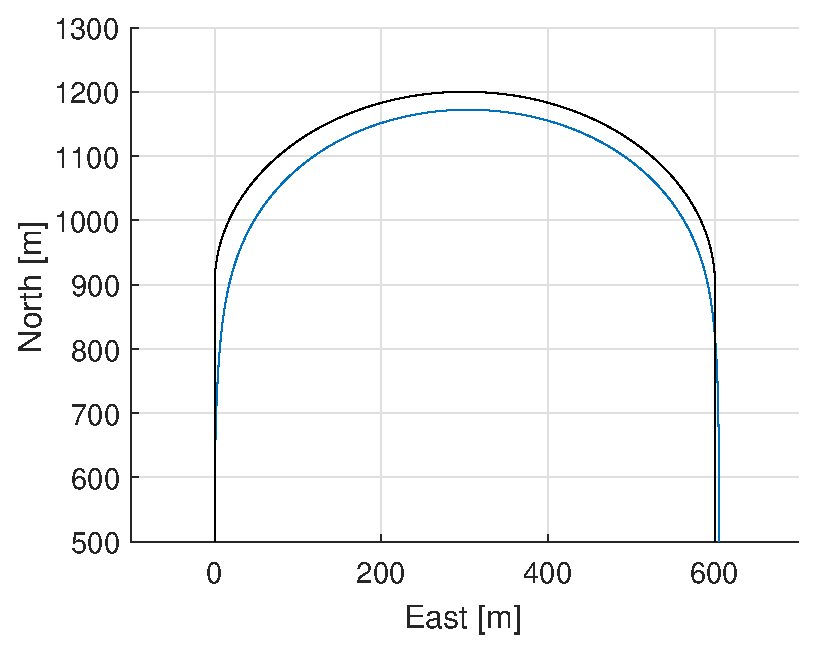
\includegraphics[width=0.5\textwidth, keepaspectratio=true]{../../results/opt/turns/curved/fig_180deg/uav_position_300m.eps}}
	\qquad
	\subfloat[$250$m][$250$m]{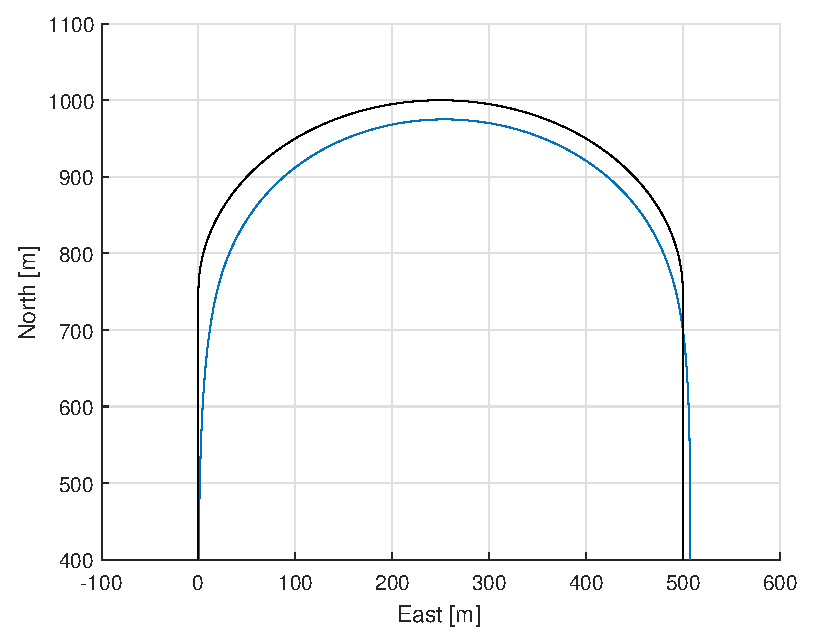
\includegraphics[width=0.5\textwidth, keepaspectratio=true]{../../results/opt/turns/curved/fig_180deg/uav_position_250m.eps}}}
	\makebox[\textwidth][c]{
	\subfloat[$200$m][$200$m]{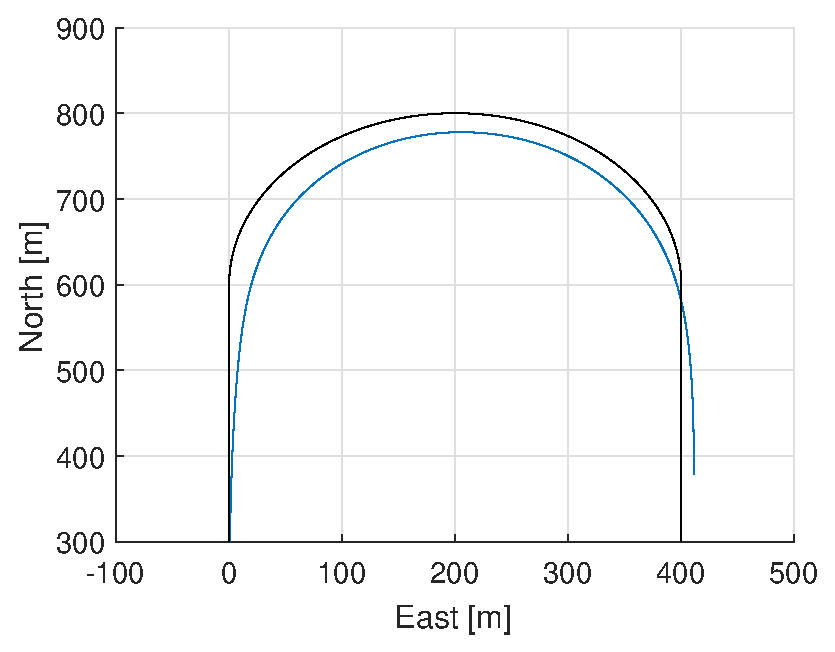
\includegraphics[width=0.5\textwidth, keepaspectratio=true]{../../results/opt/turns/curved/fig_180deg/uav_position_200m.eps}}
	\qquad
	\subfloat[$150$m][$150$m]{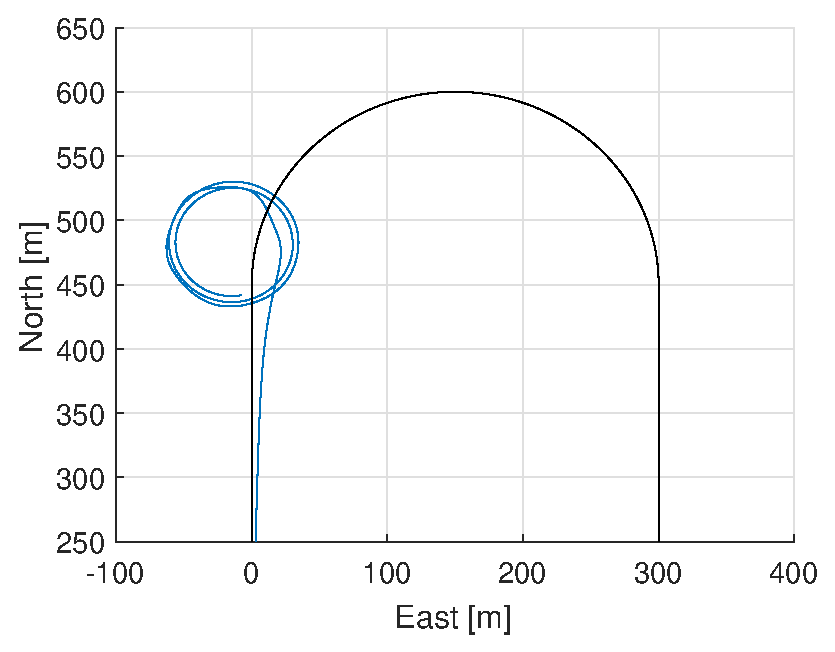
\includegraphics[width=0.5\textwidth, keepaspectratio=true]{../../results/opt/turns/curved/fig_180deg/uav_position_150m.eps}}}
	\makebox[\textwidth][c]{
	\subfloat[$100$m][$100$m]{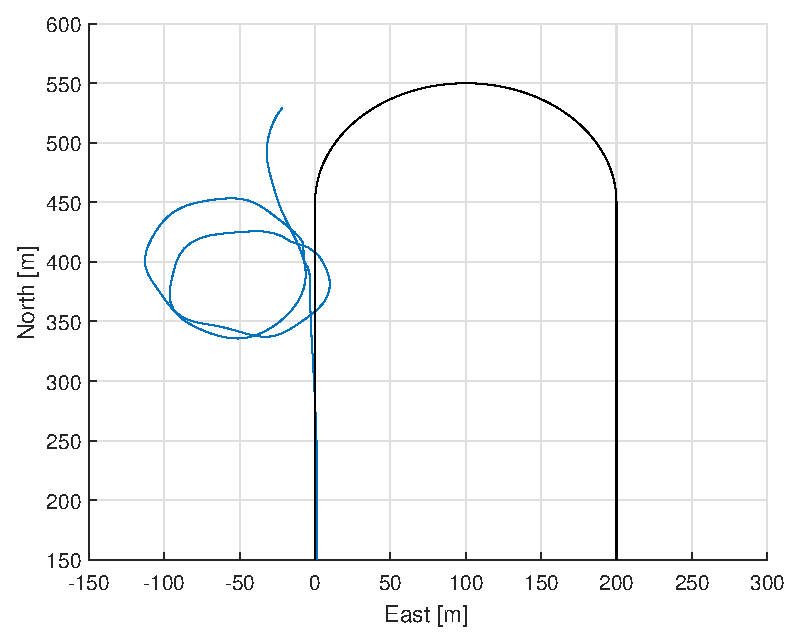
\includegraphics[width=0.5\textwidth, keepaspectratio=true]{../../results/opt/turns/curved/fig_180deg/uav_position_100m.eps}
	\label{fig:turns_cur_180deg_pos_100}}
	\qquad
	\subfloat[$50$m][$50$m]{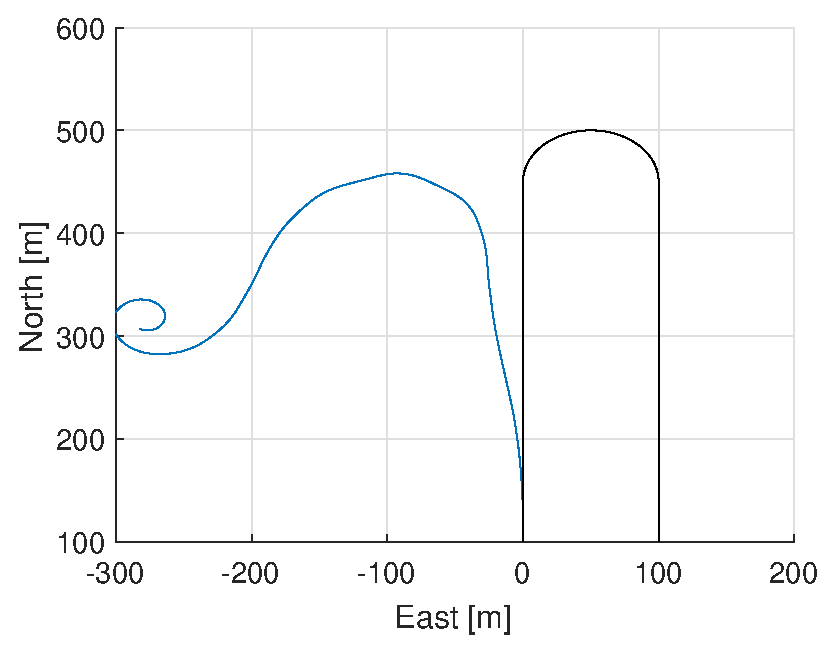
\includegraphics[width=0.5\textwidth, keepaspectratio=true]{../../results/opt/turns/curved/fig_180deg/uav_position_50m.eps}
	\label{fig:turns_cur_180deg_pos_50}}}
	\caption{The position of the UAV when optimizing a curved $180\degree$ turn with varying radius.}
	\label{fig:turns_cur_180deg_pos}
\end{figure}

\begin{figure}
	\makebox[\textwidth][c]{
	\subfloat[$300$m][$300$m]{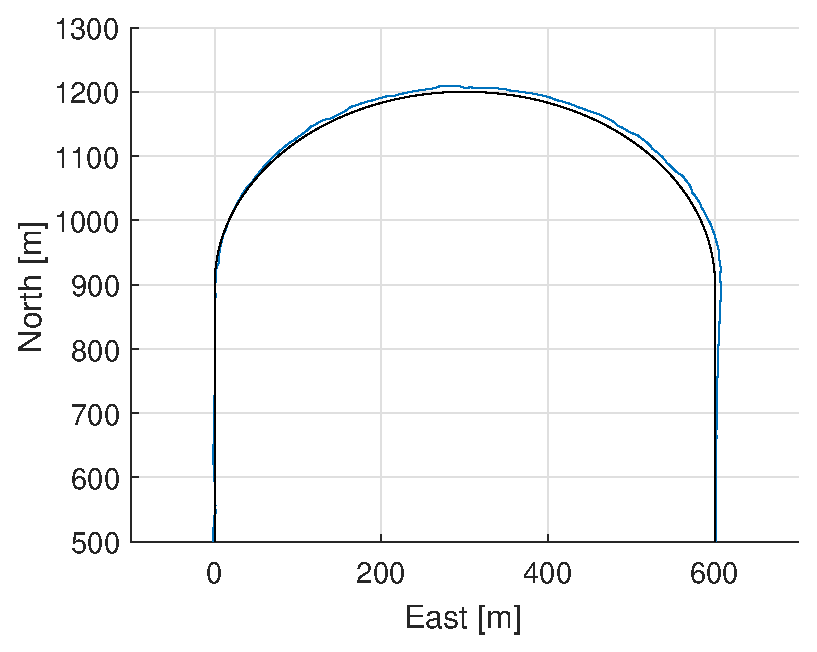
\includegraphics[width=0.5\textwidth, keepaspectratio=true]{../../results/opt/turns/curved/fig_180deg/camera_position_300m.eps}}
	\qquad
	\subfloat[$250$m][$250$m]{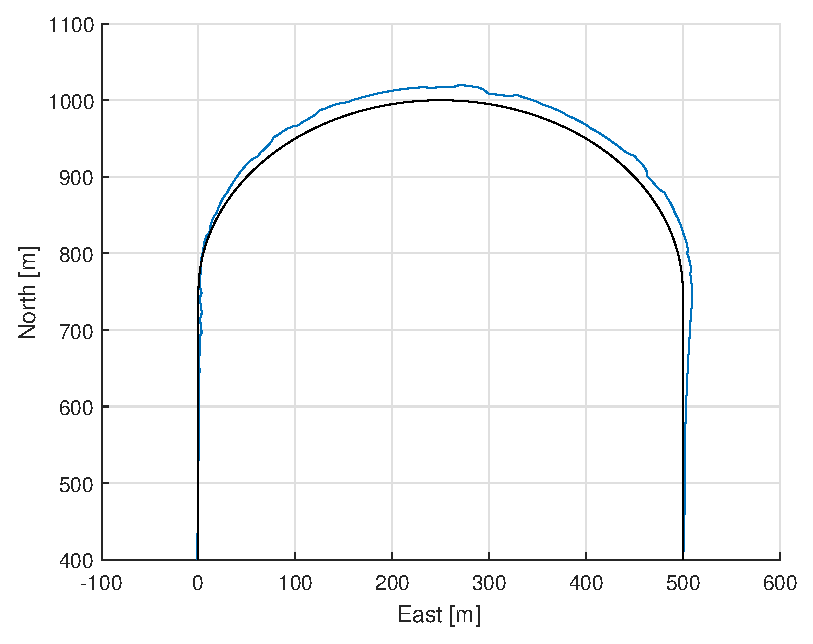
\includegraphics[width=0.5\textwidth, keepaspectratio=true]{../../results/opt/turns/curved/fig_180deg/camera_position_250m.eps}
	\label{fig:turns_cur_180deg_camera_250}}}
	\makebox[\textwidth][c]{
	\subfloat[$200$m][$200$m]{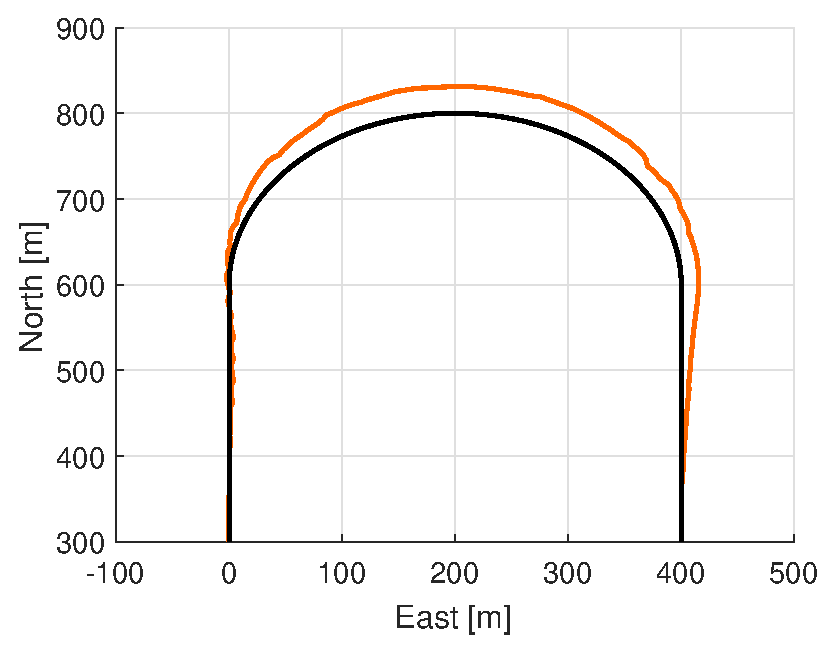
\includegraphics[width=0.5\textwidth, keepaspectratio=true]{../../results/opt/turns/curved/fig_180deg/camera_position_200m.eps}
	\label{fig:turns_cur_180deg_camera_200}}
	\qquad
	\subfloat[$150$m][$150$m]{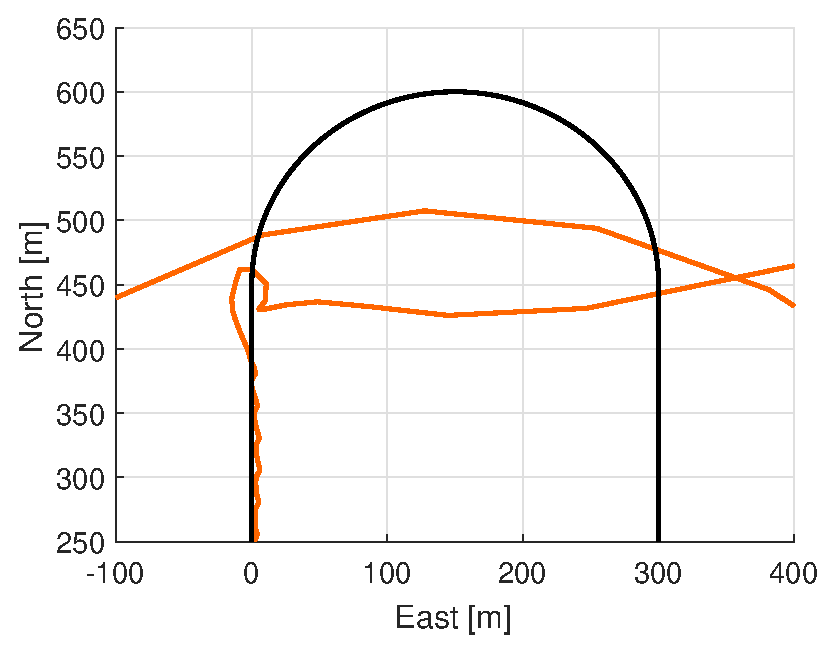
\includegraphics[width=0.5\textwidth, keepaspectratio=true]{../../results/opt/turns/curved/fig_180deg/camera_position_150m.eps}}}
	\makebox[\textwidth][c]{
	\subfloat[$100$m][$100$m]{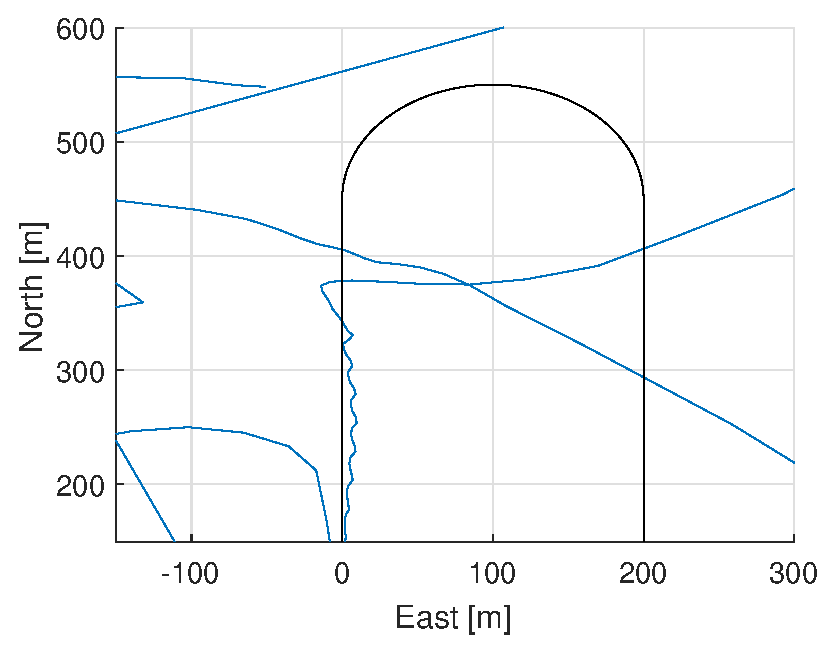
\includegraphics[width=0.5\textwidth, keepaspectratio=true]{../../results/opt/turns/curved/fig_180deg/camera_position_100m.eps}}
	\qquad
	\subfloat[$50$m][$50$m]{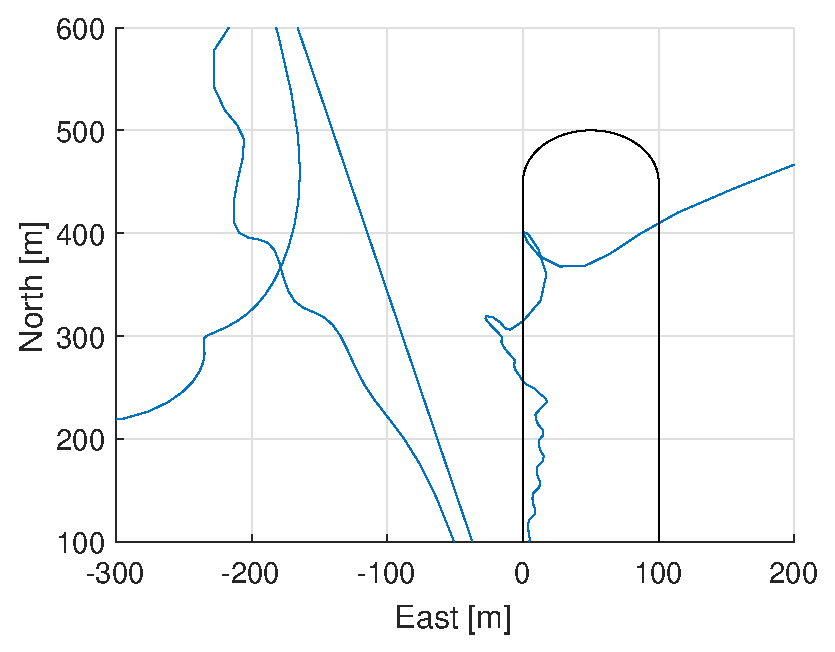
\includegraphics[width=0.5\textwidth, keepaspectratio=true]{../../results/opt/turns/curved/fig_180deg/camera_position_50m.eps}
	\label{fig:turns_cur_180deg_camera_50}}}
	\caption{The position of the camera when optimizing a curved $180\degree$ turn with varying radius.}
	\label{fig:turns_cur_180deg_camera}
\end{figure}

\begin{figure}
	\makebox[\textwidth][c]{
	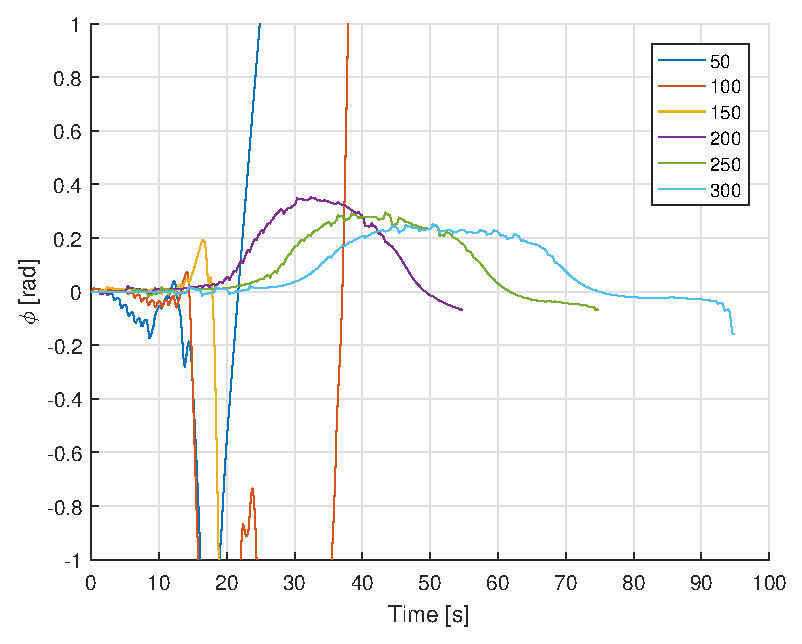
\includegraphics[width=0.8\textwidth, keepaspectratio=true]{../../results/opt/turns/curved/fig_180deg/attitude.eps}}
	\caption{The roll angle $\phi$ during the $180\degree$ turns.}
	\label{fig:turns_cur_180deg_roll}
\end{figure}